\begin{tikzpicture}[thick,scale=0.6, every node/.style={scale=0.6}]

	\onslide<1->{ % node[below=2]

		\node [text width = 20mm] (F) at (-6.5,7.5) {Input};
		\node[inner sep=0pt] (A) at (-7,6)
		{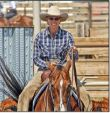
\includegraphics[scale=0.8]{images/cowboy.JPG}};
		\draw[draw=gray,fill=gray,opacity=0.5,thick,solid,rounded corners] (-8.5,4.5) rectangle (-5.5,8);   
       
	}

	\onslide<1->{

		\node [text width = 30mm] (F) at (-2.7,7.5) {Region Proposals};
		\node[inner sep=0pt] (B) at (-3.5,6)
		{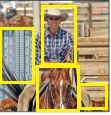
\includegraphics[scale=0.8]{images/c2.jpg}};
		\draw[black, thick, ->] (A) -- (B);     

		\node[inner sep=0pt] (C) at (-1.5,6)
		{
\includegraphics[]{images/c2_crop.jpg}};
		\draw[black,dashed, thick, ->] (-3,6.8) -- (C);     
		\draw[gray,dashed,->] (-3,6) -- (C);      
		\draw[gray,dashed,->] (-3,5) -- (C);     
		\draw[draw=gray,fill=gray,opacity=0.5,thick,solid,rounded corners] (-5,4.5) rectangle (-0.8,8);     
	}

	\onslide<1->{
		\draw[draw=blue!50,fill=yellow,thick,solid,rounded corners] (-0.4,4.5) rectangle (3.2,8);
		\node [text width = 30mm] (F) at (1.5,7.5) {Feature Extraction};
		\node[inner sep=0pt] (D) at (1.4,6)
		{\begin{tikzpicture}[thick,scale=0.6, every node/.style={scale=0.6}]     
			\pgfsetxvec{\pgfpoint{1cm}{0cm}}
			\pgfsetyvec{\pgfpoint{0cm}{1cm}}
			\pgfsetzvec{\pgfpoint{-0.707cm}{.707cm}}     
   
			\onslide<1->{
				\cuboid{(5.9,-2,0.2)}{pink!50}{0.8}{0.8}{0}
				\cuboid{(5.9,-2,0.0)}{pink!50}{0.8}{0.8}{0}
				\cuboid{(5.9,-2,-0.2)}{pink!50}{0.8}{0.8}{0}
				\cuboid{(5.9,-2,-0.4)}{pink!50}{0.8}{0.8}{0}
				\cuboid{(5.9,-2,-0.6)}{pink!50}{0.8}{0.8}{0}
				\cuboid{(5.9,-2,-0.8)}{pink!50}{0.8}{0.8}{0}
				\cuboid{(5.9,-2,-1)}{pink!50}{0.8}{0.8}{0}
				\cuboid{(5.9,-2,-1.2)}{pink!50}{0.8}{0.8}{0}
				\cuboidlabelmine{(5.9,-2,-1.2)}{pink!50}{0.8}{0.8}{0}{10}{10}{}
			}
			\onslide<1->{
         
				\cuboid{(7.9,-2.7,0.8)}{blue!50}{0.5}{0.5}{0}
				\cuboid{(7.9,-2.7,0.6)}{blue!50}{0.5}{0.5}{0}
				\cuboid{(7.9,-2.7,0.4)}{blue!50}{0.5}{0.5}{0}
				\cuboid{(7.9,-2.7,0.2)}{blue!50}{0.5}{0.5}{0}
				\cuboid{(7.9,-2.7,-0.0)}{blue!50}{0.5}{0.5}{0}
				\cuboid{(7.9,-2.7,-0.2)}{blue!50}{0.5}{0.5}{0}
				\cuboid{(7.9,-2.7,-0.4)}{blue!50}{0.5}{0.5}{0}
				\cuboid{(7.9,-2.7,-0.6)}{blue!50}{0.5}{0.5}{0}
				\cuboidlabelmine{(7.9,-2.7,-0.6)}{blue!50}{0.5}{0.5}{0}{5}{5}{}
				\kernel{(6.1,-3,-0.4)}{gray}{0.2}{0.2}{0}{(7.8,-3.2,-0.4)}
			}
			\onslide<1->{
         
				\cuboid{(9.8,-3.5,1.8)}{magenta!50}{0.5}{0}{1.4}
				%   \node at (9.3,-2.85,2.2) {\tiny{FC 1}};
				\draw[black] (7.9,-2.7,0.8) -- (9.55,-3.5,1.78);
				\draw[black] (7.9,-2.7,-0.6) -- (8.8,-3,-0.3);
			}
			\onslide<1->{
				\cuboid{(10.8,-3.5,1.7)}{magenta!50}{0.5}{0}{1.15}
         
				\draw[black] (9.8,-3.5,1.8) -- (10.5,-3.5,1.7);
				\draw[black] (9.8,-3.5,0.4) -- (10.3,-3.5,0.55);
			}
		\end{tikzpicture}};
		\draw[black, thick, ->] (C) -- (D);          
	}
	
	\onslide<1->{
	
		\tikzstyle{input_neuron}=[circle,draw=red!50,fill=red!10,thick,minimum size=6mm]
		\tikzstyle{hidden_neuron}=[circle,draw=blue!50,fill=cyan!10,thick,minimum size=6mm]
		\tikzstyle{output_neuron}=[circle,draw=green!50,fill=green!10,thick,minimum size=6mm]
		\tikzstyle{cpy_neuron}=[circle,draw=red!50,fill=red!50,thick,minimum size=6mm]
		\tikzstyle{input}=[circle,draw=black!50,fill=black!20,thick,minimum size=6mm]
	
		
		\node [text width = 30mm] (F) at (5.3,9.5) {Classifier};
		%    \draw (4.5,6.5) rectangle (6.5,8);
		%\node [text width = 25mm] (E) at (4.5,8.2) {Linear Classifier};
		\draw  (3.8,7.85) -- (3.8,9.1);
		\draw  (3.8,7.8) -- (5.2,7.8);
		\node[inner sep=0pt] (I) at (4.5,8.5)
		{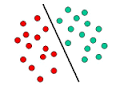
\includegraphics[scale = 0.4,trim={0.5cm 0 0.5cm 0},clip]{images/svm.png}};
	
		\draw[red!100,fill=red!10,thick,solid,rounded corners=10pt] (6,6.7) rectangle (7,9.8);
	
		\node [hidden_neuron] (neuron51) at (6.5,9.2) {} ;
		\node [hidden_neuron] (neuron52) at (6.5,8.5)  {};
		\node at (6.5,7.9) {\vdots};
		\node [hidden_neuron] (neuron53) at (6.5,7.2)  {};
		\node [cpy_neuron] (neuron01) at (6.5,8.5) {};
	
		\draw [->] (I) -- (neuron01);
		\draw  (2.7,6) -- (2.7,7);
		\draw  (2.7,7) -- (4.2,7);
		\draw [->]  (4.2,7) -- (4.2,7.8);
		\draw[draw=gray,fill=gray,opacity=0.5,thick,solid,rounded corners] (3.6,10) rectangle (7.2,6.5);
	}
	
	
	\onslide<1->{
	
		
		\node [text width = 30mm] (F) at (5.3,5.6) {Bounding Box Regression};
	
		\node[inner sep=0pt] (A) at (5.2,4.2)
		{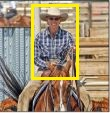
\includegraphics[scale = 0.6]{images/cowboy_cr.jpg}};
	
		\draw  (1.6,5.5) -- (1.6,4);
		\draw [->] (1.6,4) -- (4.2,4);
		\draw[draw=gray,fill=gray,opacity=0.5,thick,solid,rounded corners] (3.6,3.1) rectangle (7.2,6.2);   
	}

\end{tikzpicture}